%%%%%%%%%%%%%%%%%%%%%%%%%%%%%%%%%%%%%%%%%%%%%%%%%
%%%%%%%%%%%%%%%%%%%%%%%%%%%%%%%%%%%%%%%%%%%%%%%%%
\chapter{Results}
\label{chap:results}
Section \ref{overview} focuses on providing a general overview of algorithm performances, and the motivation for the development of an algorithm that can adapt to item type ratio is presented in section \ref{relationship}. Section \ref{Adaptability} highlights how efficiently the honey bee algorithm adapts to item type ratio. %Analysis of the other performance measures, a discussion of the performance per individual environment type,  as well as scalability study for grid sizes, number of robots and percentage of objects, will be left for a future publication. 

\subsection{General Overview}
\label{overview}
When comparing two foraging algorithms, a pairwise Wilcoxon test was performed to determine if a statistical difference occurs, at a significance level of 95\%. The test was performed over all environments. The null  hypothesis is that the results of the two algorithms come from the same distribution. Table \ref{summarytable} gives a final algorithm ranking where 2 is the best performing algorithm and 0 is the worst performing algorithm.


\vspace{-2em}
\begin{table}
\centering
    \caption{The overall Pairwise Mann Whitney U ranking, averages and standard deviations of for $\sigma$ for each algorithm}
        \label{summarytable}
    \begin{tabular}{l|lll}
    \hline \hline
    Algorithms & Wins & Average & Std Dev \\ \hline
    Naive      & 0    & 0.528   & 0.394  \\
    Desert Ant  & 1    & 0.643   & 0.387  \\
    Honey Bee   & 2    & 0.807   & 0.294  \\

    \hline
    \end{tabular}

\end{table}
Statistical tests indicate a significant difference between the results of all algorithms. Desert ant foraging performed better than na\"ive foraging showing the positive effect of site fidelity. The honey bee algorithm out-performed the na\"ive foraging algorithm and desert ant algorithm indicating the positive effect of communication and adaptivity of the honey bee foraging algorithm. The standard deviation is high for all algorithms due to the extremely large variations in the environments provided.

\subsection{Analysis of Relationship between Item Ratio in Environment and Item Ratio of Robots}
\label{relationship}

The following hypotheses are addressed:
\begin{enumerate}
\item An algorithm that forages a portion of non-prioritized items will have greater performance than an algorithm that does not forage any non-prioritized items.
\item Algorithm performance depends on the $r$ as well as $\tau$ and that as $r$ increases, the value of $\tau$ that yields the greatest value of $\sigma$, $\tau_{best}$, will increase approximately linearly for the na\"ive and desert ant algorithms.
\end{enumerate}

An algorithm configured with $\tau=1$ is where only prioritized items are foraged. Analysing Table \ref{ratio}, for the na\"ive and desert ant algorithms, for all values of $r$ where $r \neq 1$, $\tau_{best}$ is never equal to $1$, proves the hypothesis that the algorithms achieved the best performance when some robots are configured to forage non-prioritized items. The result may be because non-prioritized items are moved out of the way to allow for easier, faster access to prioritized items or allow access to inaccessible prioritized items.


\begin{table} [h]
     \caption{The performance, $\sigma$, for each foraging algorithm, for each combinations of $r$ and $\tau$. If $\tau_{best}$ exists, $\tau_{best}$ is provided. The best value of $\sigma$ is shown in bold.}
     \label{ratio}
	\centering
    \begin{tabular}{|c|c||l|l|l|l|l|l|l|l|l||l|}
	\hline    & & \multicolumn{9}{ |c|| } {$\tau$} &   \\ 
    \cline{3-11}
\multirow{-2}{*}{Algorithm}  &  \multirow{-2}{*}{$r$} & 0     & 0.2   & 0.25  & 0.333 & 0.5   & 0.667  & 0.75  & 0.8    & 1   & \multirow{-2}{*}{$\tau_{best}$ } \\ \hline
    &0     & 1 & 1     & 1     & 1     & 1     & 1     & 1     & 1     & 1     & \\
    &0.2   & 0 & 0.492 & 0.526 & 0.567 & \textbf{0.597} & 0.595 & 0.587 & 0.577 & 0.471 & 0.5 \\
    &0.25  & 0 & 0.484 & 0.526 & 0.557 & 0.588 & \textbf{0.595} & 0.585 & 0.575 & 0.477 & 0.667\\
    &0.333 & 0 & 0.467 & 0.507 & 0.544 & 0.586 & \textbf{0.596} & 0.592 & 0.584 & 0.495 & 0.667\\
    &0.5   & 0 & 0.428 & 0.46  & 0.508 & 0.568 & 0.588 & \textbf{0.591} & 0.589 & 0.528 & 0.75\\
    &0.667 & 0 & 0.4   & 0.433 & 0.487 & 0.544 & 0.583 & \textbf{0.591} & 0.593 & 0.554 & 0.75 \\
    &0.75  & 0 & 0.377 & 0.425 & 0.47  & 0.531 & 0.576 & 0.585 & \textbf{0.591} & 0.567 & 0.8\\
    &0.8   & 0 & 0.372 & 0.409 & 0.455 & 0.53  & 0.571 & 0.584 & \textbf{0.592} & 0.575 & 0.8\\
\multirow{-9}{*}{Na\"ive}&    1     & 0 & 0.336 & 0.375 & 0.433 & 0.5   & 0.552 & 0.57  & 0.581 & \textbf{0.618} & 1\\
     \hline
 &   0                    & 1 & 1     & 1     & 1     & 1     & 1     & 1     & 1     & 1       &    \\
&    0.2                  & 0 & 0.698 & 0.724 & \textbf{0.737} & \textbf{0.737} & 0.712 & 0.694 & 0.67  & 0.519 & 0.333\\
&    0.25                 & 0 & 0.678 & 0.711 & 0.73  & \textbf{0.735} & 0.715 & 0.697 & 0.673 & 0.530 & 0.5 \\
&    0.333                & 0 & 0.65  & 0.693 & 0.722 & \textbf{0.739} & 0.725 & 0.71  & 0.686 & 0.562 & 0.5\\
&    0.5                  & 0 & 0.596 & 0.645 & 0.684 & 0.729 & \textbf{0.734} & 0.725 & 0.701 & 0.621 & 0.667\\
&    0.667                & 0 & 0.554 & 0.607 & 0.648 & 0.706 & 0.737 & \textbf{0.738} & 0.716 & 0.675 & 0.75\\
&    0.75                 & 0 & 0.533 & 0.587 & 0.63  & 0.691 & 0.731 & \textbf{0.739} & 0.72  & 0.703  & 0.75 \\
&    0.8                  & 0 & 0.523 & 0.577 & 0.62  & 0.682 & 0.725 & 0.736 & \textbf{0.74}  & 0.718 & 0.8\\
\multirow{-9}{*}{Desert Ant}&    1                    & 0 & 0.488 & 0.543 & 0.588 & 0.654 & 0.702 & 0.718 & 0.726 & \textbf{0.758} & 1\\ \hline
    %Honey Bee
&        0  & 1     & 1     & 1     & 1     & 1     & 1     & 1     & 1     & 1  &   \\
&    0.2                  & \textbf{0.687} &\textbf{0.687} & 0.686 & 0.686 & 0.686 & 0.685 & 0.686 & 0.685 & \textbf{0.687} &\\
&    0.25                 & 0.678 & \textbf{0.679} & 0.678 & 0.678 &\textbf{0.679} & \textbf{0.679} & 0.678 & 0.677 & \textbf{0.679} &\\
&    0.333                & \textbf{0.674} & \textbf{0.674} & \textbf{0.674} & \textbf{0.674} & \textbf{0.674} & \textbf{0.674} & 0.673 & \textbf{0.674} &\textbf{0.674} &\\
&    0.5                  & 0.668 & \textbf{0.669} & 0.668 & 0.668 & 0.668 & 0.668 & 0.668 & 0.668 & \textbf{0.669} &\\
&    0.667                & 0.671 & 0.671 & 0.671 & 0.671 & 0.671 & \textbf{0.672} & 0.671 & 0.671 & 0.671 &\\
&    0.75                 & 0.672 & \textbf{0.673} & 0.671 & 0.671 & 0.672 &\textbf{0.673} & 0.672 & \textbf{0.673} & \textbf{0.673}&\\
&    0.8                  & 0.674 & 0.674 & 0.674 & 0.674 & 0.674 & \textbf{0.675} &  \textbf{0.675} &  \textbf{0.675} & \textbf{0.675}& \\
\multirow{-9}{*}{Honey Bee}&    1                    & \textbf{0.691} & 0.69  & \textbf{0.691} & 0.69  & \textbf{0.691} &  \textbf{0.691}& 0.69  & 0.69  & 0.69  &\\ \hline

    \end{tabular}

\end{table}

Fig \ref{desertantplot} shows the region in parameter space where the desert ant algorithm performs the best. The na\"ive and desert ant algorithms performed best when $\tau$ was slightly greater than $r$. The existence of the relationship motivates the development of an algorithm that adapts $\tau$ to correspond the environment item ratio $r$.

\begin{figure}[!htb]
\centering
\resizebox{0.8\textwidth}{!}{% GNUPLOT: LaTeX picture with Postscript
\begingroup
  \makeatletter
  \providecommand\color[2][]{%
    \GenericError{(gnuplot) \space\space\space\@spaces}{%
      Package color not loaded in conjunction with
      terminal option `colourtext'%
    }{See the gnuplot documentation for explanation.%
    }{Either use 'blacktext' in gnuplot or load the package
      color.sty in LaTeX.}%
    \renewcommand\color[2][]{}%
  }%
  \providecommand\includegraphics[2][]{%
    \GenericError{(gnuplot) \space\space\space\@spaces}{%
      Package graphicx or graphics not loaded%
    }{See the gnuplot documentation for explanation.%
    }{The gnuplot epslatex terminal needs graphicx.sty or graphics.sty.}%
    \renewcommand\includegraphics[2][]{}%
  }%
  \providecommand\rotatebox[2]{#2}%
  \@ifundefined{ifGPcolor}{%
    \newif\ifGPcolor
    \GPcolorfalse
  }{}%
  \@ifundefined{ifGPblacktext}{%
    \newif\ifGPblacktext
    \GPblacktexttrue
  }{}%
  % define a \g@addto@macro without @ in the name:
  \let\gplgaddtomacro\g@addto@macro
  % define empty templates for all commands taking text:
  \gdef\gplbacktext{}%
  \gdef\gplfronttext{}%
  \makeatother
  \ifGPblacktext
    % no textcolor at all
    \def\colorrgb#1{}%
    \def\colorgray#1{}%
  \else
    % gray or color?
    \ifGPcolor
      \def\colorrgb#1{\color[rgb]{#1}}%
      \def\colorgray#1{\color[gray]{#1}}%
      \expandafter\def\csname LTw\endcsname{\color{white}}%
      \expandafter\def\csname LTb\endcsname{\color{black}}%
      \expandafter\def\csname LTa\endcsname{\color{black}}%
      \expandafter\def\csname LT0\endcsname{\color[rgb]{1,0,0}}%
      \expandafter\def\csname LT1\endcsname{\color[rgb]{0,1,0}}%
      \expandafter\def\csname LT2\endcsname{\color[rgb]{0,0,1}}%
      \expandafter\def\csname LT3\endcsname{\color[rgb]{1,0,1}}%
      \expandafter\def\csname LT4\endcsname{\color[rgb]{0,1,1}}%
      \expandafter\def\csname LT5\endcsname{\color[rgb]{1,1,0}}%
      \expandafter\def\csname LT6\endcsname{\color[rgb]{0,0,0}}%
      \expandafter\def\csname LT7\endcsname{\color[rgb]{1,0.3,0}}%
      \expandafter\def\csname LT8\endcsname{\color[rgb]{0.5,0.5,0.5}}%
    \else
      % gray
      \def\colorrgb#1{\color{black}}%
      \def\colorgray#1{\color[gray]{#1}}%
      \expandafter\def\csname LTw\endcsname{\color{white}}%
      \expandafter\def\csname LTb\endcsname{\color{black}}%
      \expandafter\def\csname LTa\endcsname{\color{black}}%
      \expandafter\def\csname LT0\endcsname{\color{black}}%
      \expandafter\def\csname LT1\endcsname{\color{black}}%
      \expandafter\def\csname LT2\endcsname{\color{black}}%
      \expandafter\def\csname LT3\endcsname{\color{black}}%
      \expandafter\def\csname LT4\endcsname{\color{black}}%
      \expandafter\def\csname LT5\endcsname{\color{black}}%
      \expandafter\def\csname LT6\endcsname{\color{black}}%
      \expandafter\def\csname LT7\endcsname{\color{black}}%
      \expandafter\def\csname LT8\endcsname{\color{black}}%
    \fi
  \fi
  \setlength{\unitlength}{0.0500bp}%
  \begin{picture}(7200.00,5040.00)%
    \gplgaddtomacro\gplbacktext{%
      \csname LTb\endcsname%
      \put(946,704){\makebox(0,0)[r]{\strut{} 0.2}}%
      \put(946,1213){\makebox(0,0)[r]{\strut{} 0.3}}%
      \put(946,1722){\makebox(0,0)[r]{\strut{} 0.4}}%
      \put(946,2231){\makebox(0,0)[r]{\strut{} 0.5}}%
      \put(946,2740){\makebox(0,0)[r]{\strut{} 0.6}}%
      \put(946,3248){\makebox(0,0)[r]{\strut{} 0.7}}%
      \put(946,3757){\makebox(0,0)[r]{\strut{} 0.8}}%
      \put(946,4266){\makebox(0,0)[r]{\strut{} 0.9}}%
      \put(946,4775){\makebox(0,0)[r]{\strut{} 1}}%
      \put(1078,484){\makebox(0,0){\strut{} 0.2}}%
      \put(1794,484){\makebox(0,0){\strut{} 0.3}}%
      \put(2509,484){\makebox(0,0){\strut{} 0.4}}%
      \put(3225,484){\makebox(0,0){\strut{} 0.5}}%
      \put(3940,484){\makebox(0,0){\strut{} 0.6}}%
      \put(4656,484){\makebox(0,0){\strut{} 0.7}}%
      \put(5372,484){\makebox(0,0){\strut{} 0.8}}%
      \put(6087,484){\makebox(0,0){\strut{} 0.9}}%
      \put(6803,484){\makebox(0,0){\strut{} 1}}%
      \put(176,2739){\rotatebox{-270}{\makebox(0,0){\strut{}$\tau$}}}%
      \put(3940,154){\makebox(0,0){\strut{}$r$}}%
    }%
    \gplgaddtomacro\gplfronttext{%
      \csname LTa\endcsname%
      \put(5381,3757){\makebox(0,0)[l]{\strut{}  0.74}}%
      \csname LT0\endcsname%
      \put(5372,4688){\makebox(0,0)[l]{\strut{} 0.72}}%
      \put(6209,3503){\makebox(0,0)[l]{\strut{}  0.72}}%
      \put(1187,958){\makebox(0,0)[l]{\strut{} 0.72}}%
      \csname LT1\endcsname%
      \put(4418,4154){\makebox(0,0)[l]{\strut{} 0.7}}%
      \put(5372,2587){\makebox(0,0)[l]{\strut{}  0.7}}%
      \csname LT2\endcsname%
      \put(4418,4655){\makebox(0,0)[l]{\strut{} 0.68}}%
      \put(5469,2231){\makebox(0,0)[l]{\strut{}  0.68}}%
      \csname LT3\endcsname%
      \put(3225,4277){\makebox(0,0)[l]{\strut{}  0.66}}%
      \put(6201,2307){\makebox(0,0)[l]{\strut{}  0.66}}%
      \csname LT4\endcsname%
      \put(3225,4530){\makebox(0,0)[l]{\strut{}  0.64}}%
      \put(5372,1654){\makebox(0,0)[l]{\strut{}  0.64}}%
      \csname LT5\endcsname%
      \put(2032,4299){\makebox(0,0)[l]{\strut{}  0.62}}%
      \put(5386,1382){\makebox(0,0)[l]{\strut{}  0.62}}%
      \csname LT6\endcsname%
      \put(2032,4462){\makebox(0,0)[l]{\strut{}  0.6}}%
      \put(6267,1382){\makebox(0,0)[l]{\strut{}  0.6}}%
      \csname LT7\endcsname%
      \put(2032,4625){\makebox(0,0)[l]{\strut{}  0.58}}%
      \put(5372,986){\makebox(0,0)[l]{\strut{}   0.58}}%
      \csname LT8\endcsname%
      \put(1436,4564){\makebox(0,0)[l]{\strut{}  0.56}}%
      \put(6087,958){\makebox(0,0)[l]{\strut{}   0.56}}%
      \csname LT0\endcsname%
      \put(1436,4706){\makebox(0,0)[l]{\strut{}  0.54}}%
    }%
    \gplbacktext
    \put(0,0){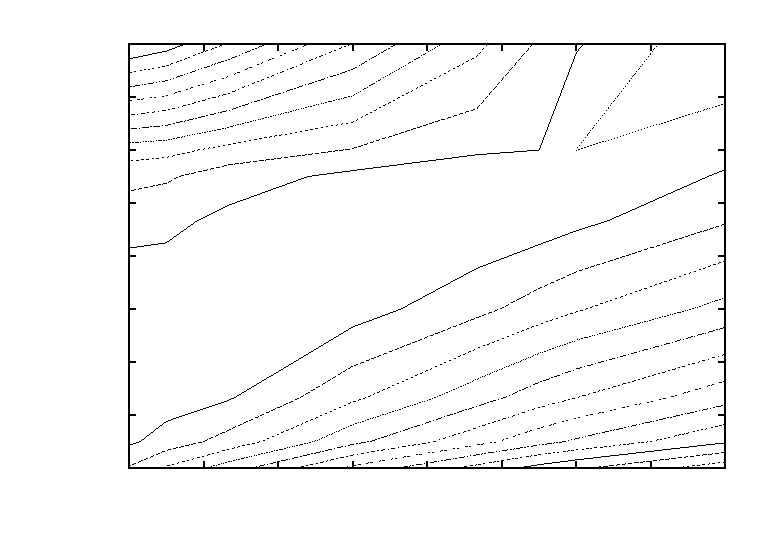
\includegraphics{chapters/chapter6/desertantplot}}%
    \gplfronttext
  \end{picture}%
\endgroup
}
\caption{Contour plot of values for $\sigma$ over values for $r$ and $\tau$ for desert ant foraging}
\label{desertantplot}
\end{figure}

 %But why? Give reason 
%The nai\"ve foraging algorithm slowly clear an entire area around the sink. If there is an equal ratio of robot types to item types then this area would be cleared effectively. 
 %fact that in the more organized environments such as gaussian or vein, it is 

\subsection{Adaptability of the Honey Bee Foraging Algorithm to Item Type Ratio and Comparison to the Na\"ive the Desert Ant Algorithms for Na\"ive and Desert Ant Algorithms}
\label{Adaptability}
Analysis of Table \ref{ratio} indicates that the honey bee foraging algorithm has similar performance throughout all configurations for $r$ and $\tau$, which highlights that the performance of the honey bee algorithm is independent of the configuration of $\tau$, resulting in an algorithm that is more flexible and robust. This could mean that the honey bee algorithm could perform well in dynamic environments where robots and items can be destroyed.

However, according to Table \ref{ratio}, the desert ant algorithm performs better than the honey bee algorithm, for particular configurations of $r$ and $\tau$. This indicates that, if the value of $r$ is known for a particular environment, then it is beneficial to use desert ant foraging and choose $\tau$ appropriately. A possible reason why the desert ant algorithm performs better when optimally configured for a particular environment than the honey bee algorithm is that the honey bee algorithm takes time to adapt to the environment, while the desert ant algorithm with optimal configurations has no division of labour overhead and may outperform the honey bee algorithm under those circumstances.


%\begin{figure}
%\input{naiveplot.tex}
%\caption{Contour plot of values for $\sigma$ over values for $r$ and $\tau$ for nai%\"ve foraging}
%\end{figure}


%\subsection{Energy}

%Due to the waiting state, the honey bee algorithm should  saving energy and thus be more energy efficient. The amount of time spent in a waiting state was measured, however surprisingly, not much time was spent waiting overall. This indicates that there is room for improvement from an energy perspective.

%%%%%%%%%%%%%%%%%%%%%%%%%%%%%%%%%%%%%%%%%%%%%%%%%
\section{Summary}
\label{results:summary}

%%%%%%%%%%%%%%%%%%%%%%%%%%%%%%%%%%%%%%%%%%%%%%%%%
%%%%%%%%%%%%%%%%%%%%%%%%%%%%%%%%%%%%%%%%%%%%%%%%%